Here we discuss modifications of the group lasso in order to deal with strongly correlated columns in $\bX$.  Our approach is motivated by the recently proposed OWL \cite{owl} norm, a special case of which is the so-called OSCAR \cite{oscar}.  These methods are designed to automatically cluster and effectively average highly correlated columns in the data matrix, and have been shown to outperform conventional lasso in many applications, particularly in cases of strong correlations. Both OWL and OSCAR deal only with the single regression setting. The main innovation here is the development of new norms, in the spirit of OWL, that allow us to deal with correlated columns in the multiple regression / multitask setting. We present two variants of the GrOWL (group OWL), and show that they  automatically group and average highly correlated columns in $\bX$ in the multiple regression setting. 

In this section, we consider the general optimization
\begin{equation}\label{eqn:L1}
\min_{\bB \in \R^{p \times r}} \ L(\bB) \ + \ G(\bB)   
\end{equation}
 where typical loss functions considered here are absolute error, $L(\bB) = \|\bY - \bX \bB \|_1$, or squared Frobenius error, $L(\bB) = \|\bY - \bX \bB \|_F^2$, and $G(\bB)$ is the GrOWL norm defined later in the section. The following results can be extended to the solution of the optimization with squared Frobenius norm loss but, for the sake of simplicity, we consider the absolute error loss in this section (details for extending the theory to Frobenius norm loss are presented in the Appendix). We give proof sketches for the main theorems and leave proofs of the theorems to the Appendix.  

\subsection{GrOWL penalty}
Let $\bB \in \R^{p\times r}$ and let $\bbeta_{i \a}$ and $\bbeta_{\a  j}$ denote the $i$th row and $j$th column of $\bB$.  Define the GrOWL penalty
\begin{equation}\label{Eqn:growl}
G(\bB) \ =  \sum_{i=1}^p w_i \|\bbeta_{[i]\a}\|_2 , 
\end{equation}
where $\bbeta_{[i]\a}$ is the row of $\bB$ with the $i$-th largest 2-norm and $\bw$ is a vector of non-negative and non-increasing weights.
Before we analyze the GrOWL regularization, we state a generalization of Lemma~2.1 in \cite{owl} which will be useful later in the section. 

\begin{lemma}\label{lemma1}
Consider a vector $\bbeta \in \R^p_+$ and any two of its components $\beta_j$ and $\beta_k$, such that $\beta_j > \beta_k$. Let $\bv \in \R^p_+$ be obtained by applying a transfer of size $\varepsilon, \varepsilon'$ to $\bbeta$ such that $\varepsilon \in (0, (\beta_j - \beta_k )/2]$ and $ -\beta_k \leq \varepsilon' \leq \varepsilon$, that is: $v_j = \beta_j - \varepsilon, v_k = \beta_k + \varepsilon'$, and $v_i = \beta_i$, for $i \neq j, k$. Let $\bw$ be a vector of non-increasing non-negative real values, $w_1 \geq w_2 \geq \cdots \geq w_p \geq 0$, and $\Delta$ be the minimum gap between two consecutive components of vector
$\bw$, that is, $\Delta = \min\{w_i - w_{i+1}, i = 1, \cdots, p - 1\}$. $\Omega_{\bw}(\cdot)$ is the OWL norm with weight vector $\bw$, then
$$\Omega_{\bw}(\bbeta) - \Omega_{\bw}(\bv) \ \geq \ \Delta \varepsilon $$
\end{lemma}

\begin{proof}
The proof is similar to that of Lemma~2.1 in \cite{owl} with different sizes $\varepsilon, \varepsilon'$ and the result follows because we assume that the increase in $k$-th component is less than the decrease in $j$-th component \ie $\varepsilon' \leq \varepsilon$.\\
More intuitively, if $\beta_k$ doesn't go up by $\varepsilon$ in magnitude, then increase its magnitude so that it does and call this $\bv'$ with $v'_j = \beta_j - \varepsilon$ and $v'_k = \beta_k + \varepsilon$.  Then we apply Lemma~2.1 in \cite{owl} to $\bv'$ and $\Omega_{\bw}(\bv) \leq \Omega_{\bw}(\bv')$. 
\end{proof}

The following theorem states that identical variables lead to equal coefficient rows corresponding to those variables in the solution given by the optimization using GrOWL.

\begin{theorem}[Identical columns]\label{ident1}
Let $\widehat \bB$ denote the solution to the optimization in (\ref{eqn:L1}) with $L(\bB) = \|\bY - \bX \bB \|_1$ or $L(\bB) = \|\bY - \bX \bB \|_F^2$.
If columns $\bx_{\a j}$ and $\bx_{\a k}$ satisfy $\bx_{\a j} = \bx_{\a k}$ and the minimum gap, $\Delta > 0$, then
$\widehat \bbeta_{j \a} = \widehat \bbeta_{k \a}$.
\end{theorem}

\textit{Proof sketch.}
The proof is divided into two steps. First, we show $\|\widehat \bbeta_{j \a}\| = \|\widehat \bbeta_{k \a}\|$ and then we further show that the rows are equal. 
We proceed by contradiction. Assume $\|\widehat \bbeta_{j \a}\| \neq \|\widehat \bbeta_{k \a}\|$ and, without loss of generality, suppose $\|\widehat \bbeta_{j \a}\| > \|\widehat \bbeta_{k \a}\|$. We see that there exists a modification of the solution with a smaller GrOWL norm using Lemma~\ref{lemma1} and same data-fitting term, and thus smaller overall objective value which contradicts our assumption that $\widehat \bB$ is the minimizer of $L(\bB) + G(\bB)$. \\

The following theorem states that nearly identical variables lead to equal norm coefficient rows corresponding to those variables in the solution given by the optimization using GrOWL.
\begin{theorem}[Correlated columns 1]\label{thm2}
Let $\widehat \bB$ denote the solution to the optimization in (\ref{eqn:L1}) with $L(\bB) = \|\bY - \bX \bB \|_1$.
If $\bx_{\a j}$ and $\bx_{\a k}$ satisfy $\|\bx_{\a j} - \bx_{\a k}\|_1 \leq \frac{\Delta}{\sqrt{r}} $, then
$\|\widehat \bbeta_{j \a}\| = \|\widehat \bbeta_{k \a}\|$.

\end{theorem}
\textit{Proof sketch.}
The proof is similar to the identical columns theorem. By contradiction and without loss of generality, suppose $\|\widehat \bbeta_{j \a}\| > \|\widehat \bbeta_{k \a}\|$. We show that there exists a transformation of $\widehat{\bB}$ such that the increase in the data fitting term is smaller than the decrease in the GrOWL norm. \\


The following theorem states that nearly identical variables lead to highly correlated coefficient rows corresponding to those variables in the solution given by the optimization using GrOWL.
\begin{theorem}[Correlated columns 2]\label{thm3}
Let $\widehat \bB$ denote the solution to the optimization in (\ref{eqn:L1}) with $L(\bB) = \|\bY - \bX \bB \|_1$.
If $\bx_{\a j}$ and $\bx_{\a k}$ satisfy $\|\bx_{\a j} - \bx_{\a k}\|_1 \leq \frac{\Delta}{\phi\sqrt{r}} $, then
$\|\widehat \bbeta_{j \a} - \widehat \bbeta_{k \a}\| \leq \frac{8\phi \|\widehat \bbeta_{k \a}\|}{4\phi^2+1}$ 
\\which further implies that 
$$1 \geq \frac{\widehat \bbeta_{j \a}^T \widehat \bbeta_{k \a}}{\|\widehat \bbeta_{j \a}\|\| \widehat \bbeta_{k \a}\|} \geq 1 - \frac{1}{2}\left( \frac{8\phi}{4\phi^2+1}\right)^2     \left( \geq 1 - \frac{2}{\phi^2}\right)$$ where $\phi \geq 1$.

\end{theorem}
\textit{Proof sketch.}
The proof is similar to the identical columns theorem. By contradiction, suppose $\|\widehat \bbeta_{j \a} - \widehat \bbeta_{k \a}\| \geq \frac{8\phi \|\widehat \bbeta_{k \a}\|}{4\phi^2+1}  \geq \frac{2 \|\widehat \bbeta_{k \a}\|}{\phi}$. We show that there exists a transformation of $\widehat{\bB}$ such that the increase in the data fitting term is smaller than the decrease in the GrOWL norm. This contradicts our assumption that $\widehat{\bB}$ is the minimizer of $L(\bB) + G(\bB)$ and completes the proof.\\

So far, we have seen that the GrOWL penalty has desirable clustering properties that lead to nearly identical coefficient rows. We study two variants of GrOWL with different weight sequences $\bw$. First, we study the weights with linear decay (equivalent to the OSCAR in single-task regression) and call it GrOWL-I. Next, we study the L1 + Linf weight sequence and call it GrOWL-II (see Figure~\ref{Fig:sim}). %We study another variant of the GrOWL which leads to exact clustering of strongly correlated columns. 

%GrOWL-I  :  $w_i = \lambda (p - i) \textnormal{ for } i = 1, \dots,  p $  

%GrOWL-II  :  $w_1 = \lambda_1 +  \lambda_2, w_i = \lambda_1, \textnormal{ for } i = 2, \dots,  p$ 
    




\iffalse
\subsection{GrOWL-2}

Let $\bB \in \R^{p\times r}$ and let $\bbeta_{i \a}$ and $\bbeta_{\a  j}$ denote the $i$th row and $j$th column of $\bB$.  Define the GrOWL norm
$$G(\bB) \ = \sum_{j=1}^r \Omega_{\bw}(\bbeta_{\a j}) \ , $$
where $\Omega_{\bw}(\cdot)$ is the OWL norm with weight vector $\bw$.  
\begin{theorem}
Let $\widehat \bB$ denote the solution to the optimization in (\ref{eqn:L1}) with $L(\bB) = \|\bY - \bX \bB \|_1$.
If $\bx_{\a j}$ and $\bx_{\a k}$ satisfy $\|\bx_{\a j}-\bx_{\a k}\|_1 \leq \Delta$, then
$\widehat \beta_{j \ell} = \widehat \beta_{k \ell}$ for $\ell = 1,\dots, r$.
\end{theorem}

\begin{proof}
The proof proceeds by contradiction.  We show that if $\widehat \beta_{j \ell} \neq \widehat \beta_{k \ell}$ for some $\ell \in \{1,\dots, r\}$, then there exists a modification of these  coefficients that reduces the OWL norm by a larger amount than the data fitting term is increased, and at the same time does not increase the group lasso norm. 

Consider the following modification.  Consider the $\ell$-th coefficient in the two rows of $\widehat \bB$ and define
$v_{j\ell} = \widehat \beta_{j \ell}-\varepsilon_\ell$ and $v_{k\ell} = \widehat \beta_{k\ell}+\varepsilon_\ell$ where $\varepsilon_\ell \ = \ (\widehat \beta_{j \ell}- \widehat \beta_{k \ell})/2 \ . $ This effectively reduces the magnitude of the larger coefficient by $|\varepsilon_\ell|$ and increases the magnitude of the other by an amount less than or equal to $|\varepsilon_\ell|$ (depending on the sign of the original coefficient).
Repeat this same sort of modification for each element in the two rows.
Define $\bV$ to have coefficients equal to those of $\widehat \bX$ except for the coefficients defined above. Using Lemma 2.1 (Pigou-Dalton transfer) in \cite{owl}, it is easy to verify that $$G(\bV) - G(\widehat\bB)  \ \leq \ -\Delta \sum_{\ell=1}^r |\varepsilon_\ell| $$

By triangle inequality, the difference in loss function $L$ that results from this modification satisfies
\begin{eqnarray*}
L(\bm V) - L(\widehat{\bm B})  & \leq  & \bigl\|{\bm x}_i - {\bm x}_j\bigr\|_1 \sum_{\ell=1}^r |\varepsilon_\ell|  \label{delta_L3}
\end{eqnarray*}
This contradicts our assumption that $\widehat{\bB}$ is the minimizer of $L(\bB) + G(\bB)$ and completes the proof.

%\textcolor{red}{This can be verified by minimizing the quantity on the right hand side with respect to $\bz$, which shows that all minimizers are proportional to $\bv$.} Triangle inequality?
%Thus it follows that 
%\begin{eqnarray*}
%\lambda \, \sum_{i=1}^p \|\bv_{i\a}\|_2  - \lambda \, \sum_{i=1}^p \|\widehat \bbeta_{i\a}\|_2  & \leq &  0
%\end{eqnarray*}
\end{proof}
\fi 

\subsection{Proximal algorithms}
We present computational algorithms for the two variants of the GrOWL norm here. The algorithms rely on the computation of the proximity operator \cite{prox} of the grOWL norm given by
\begin{eqnarray}\label{proxG}
\textnormal{prox}_{G}(\bV) = \textnormal{arg} \underset{\bB}{ \textnormal{ min } } \frac{1}{2}\|\bB - \bV\|_F^2 + G(\bB) 
\end{eqnarray}
In the following theorem, we solve for the proximity operator of grOWL in terms of the proximity of OWL. For the exact formulation of $\textnormal{prox}_{\Omega_{\bw}}$, see \cite{candes13}, \cite{ZengFigueiredo2014}.

\begin{theorem} Let $\tilde{v}_i = \| \bv_{i \a}\|$ for $i = 1, \cdots, p$. Then
$\textnormal{prox}_{G}(\bV) = \widehat \bV$, where $i$-th row of $\widehat \bV$ is
\begin{eqnarray}\label{Vhat}
\widehat \bv_{i \a} =  (\textnormal{prox}_{\Omega_{\bw}}(\tilde{\bv}))_i \frac{\bv_{i\a}}{\|\bv_{i \a}\|}
\end{eqnarray}
\end{theorem}
\textit{Proof Sketch:} The proof proceeds by finding a lower bound for the objective function in (\ref{proxG}) and then we show that the proposed solution achieves this lower bound.

%Since grOWL-2 is separable in the columns, we use the proximity of OWL, computed in \cite{candes13}, in conjunction with the SLOPE code \cite{bogdan2014} to compute the proximity of each column in parallel.

%\subsection{Simulated data results}
%In figure 1, we present a summary of simulation results comparing the estimation and prediction errors of group lasso (Glasso) and the GrOWL variants. The data is generated from the model  $\bY = \bX \bB^\star + \bW$ where $\bW$ is iid random gaussian noise with mean $0$ and variance $0.01$, the design matrix $\bX$ is also generated using random gaussian model with columns 5 and 7 set to be (nearly) identical.  We can see that for a small increase in prediction error, the grOWLs give a huge improvement in the estimation error compared to group lasso. In the following section, we see an application of these techniques to fMRI data.


\begin{figure}[!t]
    \centering
    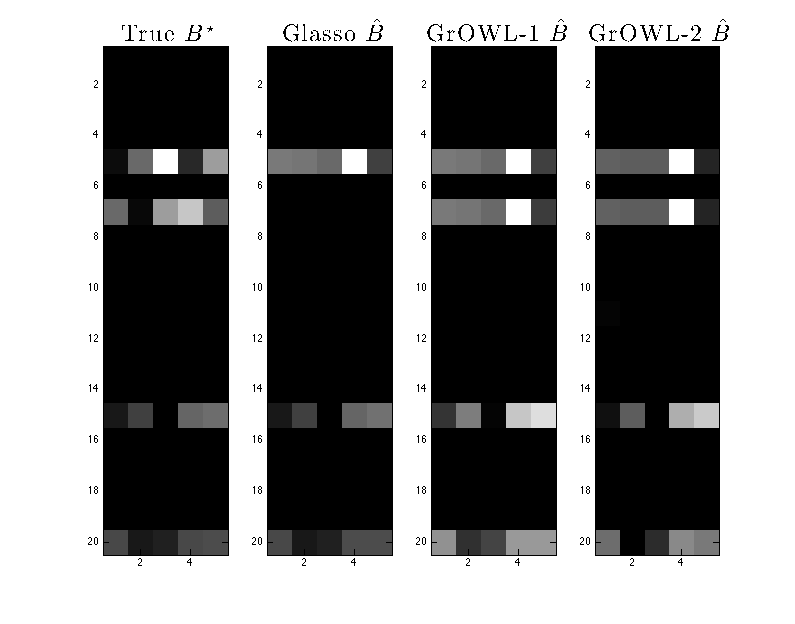
\includegraphics[width=0.9\linewidth]{figures/sim3.png}
    \qquad
    \begin{tabular}[b]{ccc}
    \hline
    	GrOWL-I:	& $w_i = \lambda (p - i) \textnormal{ for } i = 1, \dots,  p $   &\\ 
	GrOWL-II:	& $w_1 = \lambda_1 +  \lambda_2, w_i = \lambda_1 \textnormal{ for } i = 2, \dots,  p$  &\\ \hline
     % Method & Estimation error & Prediction error\\ \hline
      %Glasso & 0.638 & \textbf{0.045}\\
      %GrOWL-1 & \textbf{0.059} & 0.059\\
      %GrOWL-2 & 0.089 & 0.093\\ \hline
      %\\ 
      %\\Case 2:	& $\bbeta_{j \a}^\star \neq \bbeta_{k \a}^\star$ &
      %\\ \hline 
     % Method & Estimation error & Prediction error\\ \hline
      %Glasso & 0.753 & \textbf{0.046}\\
      %GrOWL-1 & \textbf{0.605}	 & 0.064\\
      %GrOWL-2 & 0.626 & 0.129\\ \hline
    \end{tabular}
    %\captionlistentry[table]{A comparison of solutions of group lasso and Growl optimization with correlated columns in $\bX$}
   % \captionsetup{labelformat=andtable}
    \caption{A comparison of group lasso and grOWL optimization solutions with correlated columns in $\bX$ showing that GrOWL-I and GrOWL-II select relevant features (row 5 and 7) even if they happen to be strongly correlated and automatically cluster them by setting the corresponding coefficient rows to be equal (or nearly equal).}
    \label{Fig:sim}
  \end{figure}

